\begin{chapter}{Restlessness}
    \label{chap:restlessness}

    \begin{figure}
        \centering
        
\includegraphics[width=5cm]{source/images/restlessness_logo.png}
        \caption{The Restlessness logo}
    \end{figure}

    The framework is composed by different components, listed here:
    \begin{itemize}
        \item Command Line Interface: together with the Web Interface, this is the
            main component with which users interact the most. It is available as
            the @restlessness/cli package on npm.
        \item Restlessness frontend: Web Interface with which it is possible to
            create resources and manage the project. It is part of the CLI.
        \item Restlessness backend: api service running locally, created with the
            Restlessness framework itself. It is used by the Web Interface to
            provides its functionalities.
        \item Restlessness core: core package of the framework, it contains all the
            classes and functions that provides the framework functionalities. It is
            available as @restlessness/core package on npm.
    \end{itemize}

    \section{Project creation}
    \label{sec:rln_project_creation}

    The Restlessness CLI is available for installation on the npm platform, as described
    on chapter \ref{chap:development}. % @TODO ref - be more specific after drafting the chapter
    Once installed, the first step toward using the framework is
    the creation of a new project, and that is possible using the 'new' command, as shown
    on listing \ref{lst:rln_command_new}.
    % description: creation of a new project, named rln_project
    \begin{lstlisting}[caption=New command, label={lst:rln_command_new}]
$ restlessness new rln_project
    \end{lstlisting}
    Once the command has finished, a new folder has been created, with a completely
    structured restlessness project, as can be see in figure \ref{fig:sample_rln_project_folder}.

    \begin{figure}
        \caption{Sample Restlessness project structure}
        \label{fig:sample_rln_project_folder}
        \begin{minipage}{\linewidth}
            \dirtree{%
                .1 ./.
                .2 .restlessness.json.
                .2 configs/.
                .3 authorizers.json.
                .3 daos.json.
                .3 default-headers.json.
                .3 endpoints.json.
                .3 envs.json.
                .3 models.json.
                .3 schedules.json.
                .2 envs/.
                .3 .env.locale.
                .3 .env.production.
                .3 .env.staging.
                .3 .env.test.
                .2 serverless-services/.
                .3 offline.json.
                .3 shared.json.
                .2 src/.
                .3 exporter.ts.
                .3 schedulesExporter.ts.
            }
        \end{minipage}
    \end{figure}

    The sample project shown in figure \ref{fig:sample_rln_project_folder} however,
    does not include all generated files, as some of them are not strictly part of the
    framework, but are required from other used tools, in particular:
    \begin{itemize}
        \item .eslintrc.json: configuration file of the linter
            \href{https://eslint.org/}{eslint}.
        \item .gitignore: list intentionally ignored files from the git tracking system.
        \item package.json: entry point of every npm project, it lists the project
            dependencies, as well as other project related information, such as
            the project name and version.
        \item package-lock.json: npm generated file, contains a snapshot of the
            version of all dependencies, with the goal of obtaining reproducible builds.
        \item tsconfig.json: configuration file for the Typescript compiler.
    \end{itemize}

    The first noticeable difference with respect to a plain serverless project is the
    lack of a serverless.yml (or serverless.json) file under the root.
    % @todo threshold limitation ref from chap:into and maybe also chap:aws
    In fact, due to the resource threshold limitation imposed by Aws, has been decided
    to let the framework manage the presence of multiple services inside a single
    project, so setting up a structure that is standard and micro services oriented.
    Following this structure, all serverless.yml file correspondents to the various
    services, are located under the serverless-services folder.
    Has been decided to format those configuration files using Json, instead of Yaml,
    to simplify their handling and modification by the framework, given that Typescript
    handle Json files and objects natively.
    After creation, the sample Restlessness project already contains two services,
    named shared and offline, and they are required for the framework to work.

    The shared service will contains all shared resources that can be used by all
    % (@todo ref aws api gateway description)
    the other services. This is the case for the api gateway because, since it is
    responsible for handling http requests, it is convenient to have a single url
    for all services, rather than one for each service. Other shared resources may
    be simple functions or authorizers.
    The offline service is required to handle local development, as it contains the
    resource definition of all services.
    % @todo parlare in maniera più approfondita del fatto che il servizio offline
    % deve essere trasparente per l'utente e under the hood il framework si occupa
    % di mantenere offline in sync con gli altri servizi

    Other created files are: configuration files, under the config folder, environment
    files, containing environment variables for different deployments, source code,
    under the src folder, and a .restlessness.json file, used to store project related
    information needed by the framework.

    \section{Local development}
    \label{sec:local_dev}
    The local development requires the presence of different processes, and as
    previously said, framework's side are necessary a web interface and an api
    service, and also a the project's process to be able to test it.
    The CLI handles those 3 processes through a single process, named dev (listing
    \ref{lst:rln_command_dev}).
    In particular, both the project's process and Restlessness backend, are executed
    using the Serverless plugin serverless-offline, which allow simulating an api
    gateway, effectively creating a local http server.
    Instead for the frontend process has been used the npm package serve, through
    which is possible to create an http server that serve static files.
    Furthermore the dev command takes care of executing those processes following the
    dependency order, which is: Restlessness backend, frontend and finally the
    project's process.

    % @todo schema per il processo rln che fa partire gli altri 3? see plantuml

    Another task of the dev command is to implement inter process communication between
    itself and the backend process. This is necessary as when resources are created,
    for example endpoints or schedules, the corresponding files need to be compiled by
    typescript and also the serverless-offline plugin needs to be restarted for those
    resources to be available from the http server.
    % @todo forse anche qua ci sta uno schemino

    As shown on listing \ref{lst:rln_command_dev}, the command receives the environment
    name in input, as it takes care of loading the corresponding environment variables
    from the folder .envs, as explained on section \ref{sec:env_vars}.

    \begin{lstlisting}[caption=Dev command, label={lst:rln_command_dev}]
$ restlessness dev locale
    \end{lstlisting}

    \section{Resource creation}
    The Web Interface looks like in the figure \ref{fig:rln_web_interface}, and provides
    some project details, such as serverless organization, application (section
    \ref{sec:serverless_framework}), and finally the aws data center region to which
    the project will be deployed.
    The main functionalities are then available through some shortcuts, that allow
    creating and consulting resources, such as endpoints, schedules, services and models.

    \begin{figure}
        \centering
        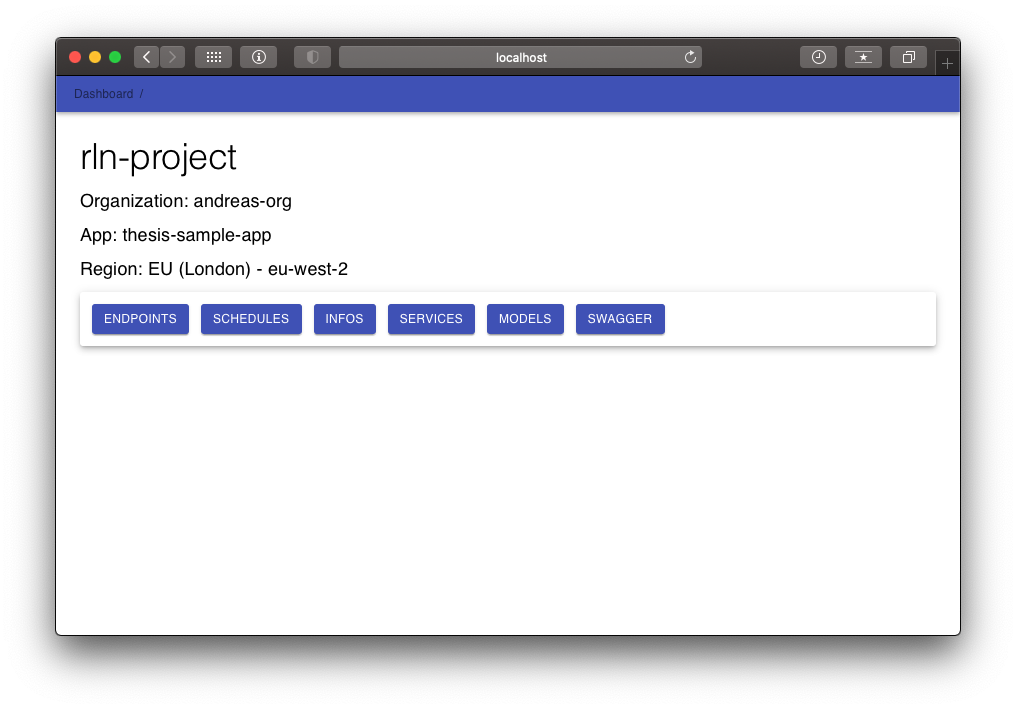
\includegraphics[width=\linewidth]{source/images/rln-web-interface.png}
        \caption{Restlessness Web Interface}
        \label{fig:rln_web_interface}
    \end{figure}

    Being Restlessness a framework for serverless services, the primary resource that
    can be defined are functions, and at the moment it is possible to define two type
    of functions, based on the event that triggers them. They are endpoints, for http
    event, and schedules, for programmed events, such as cron jobs.

    \subsection{Endpoints}
    \label{subsec:endpoints}
    It is possible to create an endpoint from the Web Interface, by specifying the
    following fields, as shown on figure \ref{fig:wi_create_endpoint}:
    \begin{itemize}
        \item Service: the service to which the function must be associated.
        \item Route: the path corresponding to the serverless function.
        \item Method: the http method.
        % \item Warmup enabled: @todo
        % \item Daos: @todo
        \item Authorizer: this optional field sets a further function, that
            perform the authorization operation, granting or denying access to
            the specified function. %, as explained on (@todo ref).
    \end{itemize}

    \begin{figure}
        \centering
        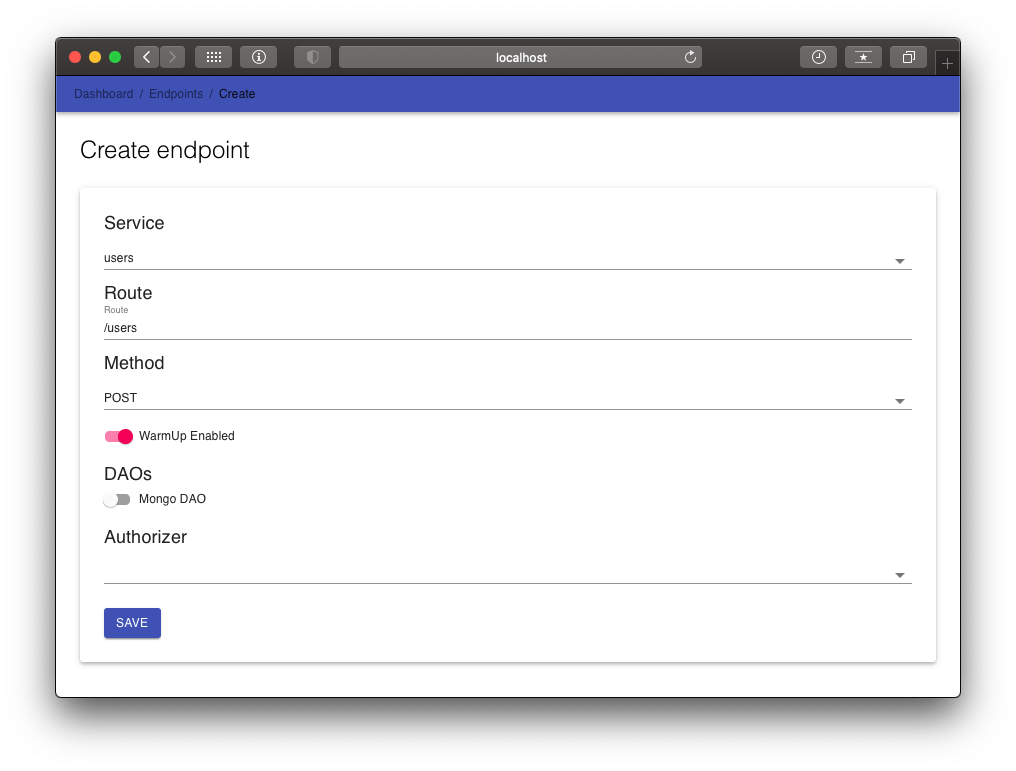
\includegraphics[width=\linewidth]{source/images/rln-wi-create-endpoint.png}
        \caption{Creation of and endpoint}
        \label{fig:wi_create_endpoint}
    \end{figure}

    During the endpoint creation, the framework takes care of saving the provided
    information on the configuration file config/endpoints.json, and to create code
    template for the development of the corresponding function.
    As shown on figure \ref{fig:new_endpoint_folder_structure}, has been created a
    folder under src/endpoints, using the notation http method plus normalized value
    of the http path.

    \begin{figure}
        \caption{Structure of a new endpoint folder}
        \label{fig:new_endpoint_folder_structure}
        \begin{minipage}{\linewidth}
            \dirtree{%
                .1 ./.
                .2 src/.
                .3 endpoints/.
                .4 post-users.
                .5 handler.ts.
                .5 index.ts.
                .5 index.test.ts.
                .5 interfaces.ts.
                .5 validations.ts.
                .3 exporter.ts.
                .3 schedulesExporter.ts.
            }
        \end{minipage}
    \end{figure}

    The developer can then code the function in handler.ts, which already contains a
    template (listing \ref{lst:handler_ts}) and define the validation object in
    validations.ts (listing \ref{lst:validations_ts}).
    It is also possible to exploit the Typescript functionalities, defining the various
    interface for the request, response and query parameters objects, all under the
    interfaces.ts file (listing \ref{lst:interfaces_ts}).
    The actual function entry point that will be executed once deployed is defined
    in the file index.ts (listing \ref{lst:index_ts}). This function is created binding
    the function LambdaHandler input with the handler function and validation object.
    LambdaHandler is a core function of the framework, its purpose is to parse the
    request payload and or query parameters, load the environment variables (section
    \ref{sec:env_vars}) and execute the lifecycle hooks of the installed addons (chapter
    \ref{chap:extensions}).
    After those operation the LambdaHandler execute the actual handler function.

    \begin{lstlisting}[caption=handler.ts content, label={lst:handler_ts}]
export default async (req: Request) => {
    try {
        const {
            validationResult,
            payload,
        } = req;

        if (!validationResult.isValid) {
            return ResponseHandler.json({
                message: validationResult.message
            }, StatusCodes.BadRequest);
        }

        return ResponseHandler.json({});
    } catch (e) {
        console.error(e);
        return ResponseHandler.json(
            {}, StatusCodes.InternalServerError);
    }
};
    \end{lstlisting}

    \begin{lstlisting}[caption=index.ts content, label={lst:index_ts}]
export default LambdaHandler
    .bind(this, handler, validations, 'postUsers');
    \end{lstlisting}

    \begin{lstlisting}[caption=validations.ts content, label={lst:validations_ts}]
const queryStringParametersValidations =
(): YupShapeByInterface<QueryStringParameters>  => ({});

const payloadValidations =
(): YupShapeByInterface<Payload> => ({});

export default () => ({
    queryStringParameters: yup.object()
        .shape(queryStringParametersValidations()),
    payload: yup.object()
        .shape(payloadValidations()).noUnknown(),
});
    \end{lstlisting}

    \begin{lstlisting}[caption=interfaces.ts content, label={lst:interfaces_ts}]
import { RequestI } from '@restlessness/core';
export interface QueryStringParameters {}
export interface Payload {}
export interface Request extends
    RequestI<QueryStringParameters, Payload, null> {};
    \end{lstlisting}

    \subsection{Schedules}
    \label{subsec:schedules}
    Schedules are serverless functions that are triggered by a programmed event,
    such as a cron job or a rate event, an event that is fired up periodically,
    based on the time interval provided.
    By creating a Schedule from the Web Interface the framework creates the necessary
    template files under src/schedules as shown on \ref{fig:new_schedule_folder_structure},
    and also save the provided information under the config/schedules.json file.

    \begin{figure}
        \caption{Structure of a schedule endpoint folder}
        \label{fig:new_schedule_folder_structure}
        \begin{minipage}{\linewidth}
            \dirtree{%
                .1 ./.
                .2 src/.
                .3 schedules/.
                .4 clean/.
                .5 handler.ts.
                .5 index.ts.
            }
        \end{minipage}
    \end{figure}

    The structure of the template files is similar to the one generated for endpoints,
    but simpler. The handler.ts file contains the function that the developer has
    to code, while the index.ts file is the entry point.
    The core function ScheduleHandler is used to wrap the handler function, the same
    way as happens for endpoints, with the purpose of executing the framework lifecycle
    hooks.

    \begin{lstlisting}[caption=handler.ts content, label={lst:sched_handler_ts}]
export default async (event) => {};
    \end{lstlisting}

    \begin{lstlisting}[caption=index.ts content, label={lst:sched_index_ts}]
import { ScheduleHandler } from '@restlessness/core';
import handler from './handler';
export default ScheduleHandler.bind(this, handler, 'clean');
    \end{lstlisting}

    % \subsection{Models}
    % \label{subsec:models}
    % @todo\\

    % parlare di come rln salva le info sulle varie risorse nei vari file
    % di configurazione
    % mostrare anche i files che vengono creati, tutta la struttura per gli
    % endpoints, per gli schedules etc...

    % descrivere come avviene internamente la creazione delle risorse, quindi
    % JsonConfigFile -> JsonEndpoints <-> JsonServices (principalmente sono quelle
    % le classi importanti)

    % The creation of a service is internally managed by the JsonServices class, which
    % provides the CRUD functionalities the the configuration file of the various
    % services defined. The creation of a service correspond to the creation of a new
    % configuration file under the serverless-services directory.

    % @todo talk about the 2 exporter files
    % qui magari mettere un class diagram

    \section{Test}
    A test template is also provided when creating a new endpoint, and it is based
    on the popular testing library \href{https://jestjs.io/}{jest}.
    % @todo talk more about the library
    In addition to the jest library, Restlessness provides also a TestHandler class,
    which makes testing the endpoint straightforward.
    Inside the beforeAll function it performs initialization operations, such as
    loading the correct environment variables, while the function invokeLambda
    executes the endpoint function providing automatically the event and context
    objects, simulating this way an http event. %  (@todo ref event and contex, aws chap)
    The fact that serverless is based on function makes possible using a simple
    testing structure as the one presented, as it's not necessary for example to
    actually starts an http server to test the endpoints.

    \begin{lstlisting}[caption=index.test.ts template, label={lst:endopints_test_ts}]
const postUsers = 'postUsers';

beforeAll(async done => {
    await TestHandler.beforeAll();
    done();
});

describe('postUsers API', () => {
    test('', async (done) => {
        const res = await TestHandler.invokeLambda(
            postUsers);
        // expect(res.statusCode).toBe(StatusCodes.OK);
        done();
    });
});

afterAll(async done => {
    await TestHandler.afterAll();
    done();
});
    \end{lstlisting}

    % \section{Api documentation}
    % @todo swagger generated documentation

    \section{Deploy}
    The Serverless Framework already provides a command for the deploy operation,
    as shown on \ref{sec:serverless_framework}, however with the micro services oriented
    structure suggested by Restlessness this operation is more elaborate, as it
    involves the deploy of more than one service, in a particular order.
    This is necessary because of the presence of the shared resources service, so
    to successfully deploy a service that uses resources from the shared one, it
    is necessary that those resources already exists. The correct deploy ordering
    is then shared service first, followed by all the other services.
    It should be noted that the offline service is not involved in the deploy
    process as it's used only for local development.
    To address this operations the Restlessness CLI provides a custom deploy
    command (listing \ref{lst:rln_command_deploy}), and a complementary remove command
    that removes all the services enforcing an opposite ordering.

    \begin{lstlisting}[caption=Deploy command, label={lst:rln_command_deploy}]
$ restlessness deploy
$ restlessness deploy --env production
$ restlessness deploy --env production users
    \end{lstlisting}

    It is possible to deploy the application on different environments, otherwise
    the command assume staging as the default environment.
    It is also possible to perform the deploy of just a single service, to keep
    the whole development, test and deploy process fast and easy, when making small
    changes, in accordance with the serverless paradigm.

    Since the deploy operation involves more than one service, it's important that
    the information between them are consistent, especially when deploying. This is
    why the deploy command, under the hood, takes care of performing this check,
    with a method from the JsonServices class, named healthCheck.
    In particular, it checks that the various services belong to the same serverless
    organization and organization, the same aws deploy region, and that do not exist
    services with functions associated to the same path. The latter is due to the fact
    that the services use a shared api gateway.

    \section{Environment variables}
    \label{sec:env_vars}
    An important aspect when developing web applications is the handling of different
    deploying environments, as each one of them requires different configurations,
    mostly for sensitive information, such as database credentials.
    Has been decided to handle this information with different environment files,
    storing environment variables.
    At project initialization the framework creates 4 different environments: locale,
    test, staging and production. Each environment has an associated type and stage.
    The type represent the purpose of that environment, beloware the available types:
    \begin{itemize}
        \item test: environments used only for testing, which can happen locally
            but also through CI platform.
        \item dev: environments used for local development
        \item deploy: environments that can be deployed
    \end{itemize}
    All information about the environments (name, type, stage) are stored in the
    configuration file config/envs.json and are managed by the JsonEnvs class.

    Environment variables are stored in the format key=value and variable expansions
    is supported, so the value of a key can be another variable, using the syntax
    shown on listing \ref{lst:env_key_syntax}.

    \begin{lstlisting}[caption=Environment variable syntax, label={lst:env_key_syntax}]
key1=${otherKey}
key2=sample ${key1}
    \end{lstlisting}

    Each environment is then stored under the envs/ directory, in the form .env.<name>,
    and the interaction with those files is handled by the EnvFile class.
    The load and expansion operation is performed differently depending on the operation,
    local development or deploy.
    During local development it is the dev command that load the environment specified
    in input (\ref{sec:local_dev}).
    During deploy instead, the environment file is expanded and copied under the
    project root, in a file named .env, as this makes deploying from CI straightforward.
    Then at runtime the .env is automatically loaded by the LambdaHandler or ScheduleHandler
    functions (\ref{subsec:endpoints}, \ref{subsec:schedules}).

\end{chapter}